\documentclass{article}
\usepackage[utf8]{inputenc}
\usepackage{amsmath}
\usepackage{upgreek}
\usepackage{amssymb}
\usepackage{graphicx}
\usepackage{float}
\usepackage{algorithm}
\usepackage{algorithmic}
\usepackage{csvsimple}

\title{Variational Inference with Coin Toss example}
\author{AntiCodeOn \\ email: {anticodeon@gmail.com}  }
\date{November 2017}


\newcommand\JointProb{p(X,Z,\Theta,\pi,a,b)}
\newcommand\Factorized{q(Z,\Theta,\pi,a,b)}
\newcommand\ProbZGivenpi{\mbox{P(Z)}}
\newcommand\ProbSingleCoin{\Theta_k^{x_n^j}(1-\Theta_k)^{1-x_n^j}}
\newcommand\ProbAllCoins{\Theta_k^{n_H}(1-\Theta_k)^{n_T}}



\newcommand\ProdK{\prod_{k=1}^{K}}
\newcommand\ProdN{\prod_{n=1}^{N}}
\newcommand\ProdJ{\prod_{j=1}^{J}}
\newcommand\SumK{\sum_{k=1}^{K}}
\newcommand\SumN{\sum_{n=1}^{N}}
\newcommand\SumJ{\sum_{j=1}^{J}}

\newcommand\Qfactor{\ProdK{q_k(z_k)}}

\DeclareMathOperator*{\argminA}{arg\,min}

\begin{document}

\maketitle

\section{Introduction}
Variational inference (VI) is a machine learning method for approximation of the difficult to compute probability densities that appear in Bayesian methods. In general, the goal is to find a surrogate distribution over hidden variables and parameters of the original Bayesian model that is close to the original distribution but where the evaluation is computationally efficient. The closeness is defined in terms of a divergence measure between the approximate distribution and the original distribution. 

\section{Motivation}
Consider classical Bayesian setup 
\begin{equation}\label{BayesEq}
p(Z|X) = \frac{p(X,Z)}{p(X)}
\end{equation}
where $X=x_{1:n}$ denotes the observed data while $Z=z_{1:k}$ denotes all the hidden variables and parameters of the model. Numerator of the fraction is called joint distribution
\begin{equation}
    p(X,Z) = p(X|Z)\:p(Z)
\end{equation}
and the denominator (often called evidence) is a marginal distribution
\begin{equation}
    p(X)=\int_{Z}p(X,Z)\:dZ
\end{equation}
Computing the posterior probability is often a very hard problem (for example, due to the exponentially large number of hidden states or because required integrations do not have a closed-form analytical solution). This is why we resort to techniques such as approximation, where the objective is to find a joint distribution $q(Z)$ that replaces original posterior $p(Z|X)$ in a way that enables us to find computationally tractable solutions.
\subsection{Variational inference setup}
Variational inference posits a set of densities $\mathcal{Q}$  over the latent variables $Z$. We typically try to minimize the Kullback-Leibler (KL) divergence
\begin{equation}\label{KL_divergence}
    KL(q(Z)\: ||\: p(Z|X)) = E_{q}\left[log\:\frac{q(Z)}{p(Z|X)}\right]
\end{equation}
of the approximate and the original, true joint distribution
\begin{equation}
    q^*(Z) = \argminA_{q(Z)\in\mathcal{Q}}\: KL(q(Z)\: ||\: p(Z|X))
\end{equation}
KL divergence tells us how much information we loose by choosing the approximate distribution instead of true posterior distribution. 
We can expand the right hand side of (\ref{KL_divergence})
\begin{equation}
KL(q(Z)\: ||\: p(Z|X)) = E_q[q(Z)] - E_q[log\:p(Z|X)]
\end{equation}
Using (\ref{BayesEq}) we get
\begin{equation}
KL(q(Z)\: ||\: p(Z|X)) = p(X) - \underbrace{(E_q[log\:p(X,Z)] - E_q[q(Z)])}_\text{ELBO(q)}
\end{equation}

We want to minimize the KL divergence by varying distribution q(Z). $p(X)$ does not depend on $q$ and is always positive (or equal to zero) so we need to maximize the $ELBO(q)$. The only assumption we are making is that $q(Z)$ factorizes in the following way 
\begin{equation}
q(Z)=\Qfactor{}
\end{equation}
which means that we are breaking possible dependencies between hidden variables in our approximation process.
\begin{equation}
    ELBO(q) = \int q(Z)\: log\:{p(X,Z)}\:dZ - \int q(Z)\:log{\:q(Z)}\:dZ
\end{equation}
In our problem we are dealing with the discrete distribution. Fortunatelly, the setup is the same, we only need to changethe integral with the summation terms.

\section{Variational inference mixture model}
For each observation $x_n$ we have a corresponding latent variable $z_n$ comprising a 1-of-K binary vector with the elements $z_{nk}$ for $k = 1, \dots, K$. We denote the observed data set by $X = {x_1, \dots, x_N}$, and similarly we denote the latent variables by $Z={z_1, \dots, z_N}$. We can write down the conditional distribution of $Z$, given the mixing coefficients $\pi$, in the form:
\begin{equation}
    p(Z|\pi) = \ProdN \ProdK \pi_k^{z_{nk}}
\end{equation}
We introduce priors over the parameter $\pi$. The mathematical analysis is considerably simplified if we choose conjugate prior distribution to model the parameter $\pi$. We choose a Dirichlet distribution over the mixing coefficients $\pi$. The parameter $\alpha$ can be interpreted as the effective prior number of observations associated with each component of the mixture. If the starting $\alpha$ value is small (bellow 1), then the posterior distribution is primarily influence by the data rather then our choise of prior.
\begin{equation}
    p(\pi) = Dir(\pi|\alpha_0) = C(\alpha_0)\ProdK{}\pi_k^{\alpha_k-1}
\end{equation}
Next, we write down the conditional distribution of the observed data vectors, given the latent variables and the component parameters. Each of the five experiments $X$ comprises of the ten independent Bernoulli events.
\begin{equation}
    p(X|Z,\Theta)= \ProdN\ProdK\ProdJ[\ProbSingleCoin{}]^{z_{nk}}
\end{equation}
We can model priors for the $\Theta$ parameter with the conjugate prior distribution of the Bernoulli distribution. As we are dealing with the coin biasses, which are defined on the interval [0, 1], beta distribution lends itself as a natural choice for our model.
\begin{equation}
    p(\Theta|a,b) = \ProdK\frac{\Theta^{a-1}(1-\Theta)^{b-1}}{Beta(a,b)}
\end{equation}
\textit{Note. The Beta in the denominator denotes the Beta function, not the Beta probability distribution}.

Joint distribution is given by
\begin{equation}\label{joint_decomp}
    \JointProb{} = p(X|Z,\Theta)p(Z|\pi)p(\pi)p(\Theta|a,b)
\end{equation}
with factors on the right side of the equation as defined above. Only variables $X={x_1,\dots,x_N}$ were observed. In the next step we consider a variational distribution with the following factorization
\begin{equation}\label{factor_decomp1}
q(Z, \pi, \Theta) = q(Z)q(\pi,\Theta).
\end{equation}
We are separating the latent variables and parameters and this is actually the only assumption we are making.
In order to proceed with the factorization, we use the general result given by Bishop[2006].
\begin{equation}
    ln\: q^*(Z)=E_{\pi,\Theta}[ln\:\JointProb] + const
\end{equation}
For the factor of \textbf{Z} we are only interested in those components of the decomposition \ref{joint_decomp} that depend on \textbf{Z}. All other terms are absorbed into the additive normalization constant, giving:
\begin{equation}
    ln\: q^*(Z)=E_{\pi}[ln\:p(Z|\pi)] + E_\Theta[ln\:p(X|Z,\Theta)] + const
\end{equation}
where
\begin{equation}
    E_{\pi}[ln\:p(Z|\pi)]  = \SumN\SumK z_{nk}E_\pi[ln\:\pi_k]
\end{equation}
and
\begin{equation}
    E_\Theta[ln\:p(X|Z,\Theta)] = \SumN\SumK z_{nk}E_\Theta[\SumJ ln\:\ProbSingleCoin]
\end{equation}
Hence
\begin{equation}
    ln\: q^*(Z)=\SumN\SumK z_{nk}\left(E_\pi[ln\:\pi_k] + E_\Theta[ln\:\ProbAllCoins]\right) + const
\end{equation}
where $n_H$ is a number of heads and $n_T$ number of tails in the n-th experiment.
Proceeding similarly for \textbf{$\pi$} and \textbf{$\Theta$} we get the following expression
\begin{equation}
    ln\: q^*(\pi,\Theta)=E_{Z}[ln\:(\pi) + ln\:p(Z|\pi)] + E_Z[ln\:p(X|Z,\Theta) + ln\:p(\Theta)] + const
\end{equation}
Since there are no expressions that depend on both parameters at the same time we may proceed with the factorization of the parameters independently
\begin{equation}\label{factor_decomp2}
    q(\pi,\Theta) = q(\pi)\:q(\Theta)
\end{equation}
where
\begin{equation}
    ln\:q^*(\pi) = ln\:p(\pi) + E_{Z}[ln\:p(Z|\pi)] + const
\end{equation}
\begin{equation}\label{factor_pi_log}
    ln\:q^*(\pi) = \SumK{(\alpha_k-1)\ln\:\pi_k} + \SumK r_k\:ln\:\pi_k+ const
\end{equation}
where $r_{k} = \SumN E[z_{nk}]$
We have already derived the expectations over $Z$ in EM document.
Taking the exponential of equation \ref{factor_pi_log} we get that the 
\begin{equation}
    q(\pi) = Dir(\pi| \upalpha)
\end{equation}
where $\upalpha$ is vector with K components $\upalpha_k = \alpha_k+r_k$

\begin{equation}
    ln\:q^*(\Theta) = ln\:p(\Theta) + E_Z[ln\:p(X|Z,\Theta)] + const
\end{equation}
\begin{equation}
    ln\:q^*(\Theta) = \SumK (ln\:[\Theta_k^{a_k-1}(1-\Theta_k)^{b_k-1}] + \SumN r_{nk}\SumJ \:ln[\Theta_k^{x_n^j}(1-\Theta_k)^{1-x_n^j}]_ + const
\end{equation}
\begin{equation}
    ln\:q^*(\Theta) = \SumK ln\:[\Theta_k^{a_k-1+\SumN n_Hr_{nk}}(1-\Theta_k)^{b_k-1+\SumN n_Tr_{nk}}] + const
\end{equation}
where $n_H$ equals number of the outcomes of $x_n^j = 1$ (number of heads), and $n_T$ number of the outcomes of $x_n^j = 0$ (number of tails).
We see that the factor for $\Theta$ is Beta distributed variable:
\begin{equation}
    q^*(\Theta) = \ProdK Beta(\Theta|A, B)
\end{equation}
where $A$ is a vector with parameter components $a = a_{k}+\SumN n_Hr_{nk}$ and $B$ with components $b = b_{k}+\SumN n_Tr_{nk}$.
\section{Variational lower bound}
Variational lower bound $L$ is given by 
\begin{equation}
    L = E[ln\:\JointProb{}] - E[ln\:\Factorized{}]
\end{equation}
Using results from \ref{joint_decomp}, \ref{factor_decomp1} and \ref{factor_decomp2}
this simplifies to
\begin{equation}
\begin{split}
    L =& E[ln\:p(X|Z,\Theta)] + E[ln\:p(Z|\pi)] + E[ln\:p(\pi)] + E[ln\:p(\Theta|a,b)] \\
    & -E[ln\:q(Z)] - E[ln\:q(\pi)] - E[ln\:q(\Theta)]
\end{split}        
\end{equation}
We write down each of the terms separately:
\begin{equation}
    E[ln\:p(\pi)] = ln\:C(\alpha_0)+\SumK (\alpha_k-1)(\psi(\alpha_k)-\psi(\SumK \alpha_k))
\end{equation}
\begin{equation}
    E[ln\:p(\Theta_k|a,b)]=\SumK -ln\:Beta(a_k,b_k)+(a_k-1)\psi(a_k)-(b_k-1)\psi(b_k)+(a_k+b_k-2)\psi(a_k+b_k)
\end{equation}
\begin{equation}
    E[ln\:p(Z|\pi) = \SumN\SumK r_{nk}(\psi(\alpha_k)-\psi(\SumK \alpha_k))
\end{equation}
\begin{equation}
    E[ln\:p(X|Z,\Theta)] = \SumN\SumK r_{nk}[n_H(\psi(a_k)-\psi(a_k+b_k))+n_T(\psi(b_k)-\psi(a_k+b_k))]
\end{equation}
\section{Algorithm}
The following table gives the algorithmic description of the problem.
\begin{algorithm}
\caption{Coordinate ascent algorithm}
\begin{algorithmic}
\REQUIRE Data $x_{1:n}$, number of components K, model
\ENSURE Variational densities q(z), q($\Theta$), q($\pi$)
\STATE \textbf{Initialize:} Variational parameters $a_{1:K}$, $b_{1:K}$, $\alpha_{1:K}$
\REPEAT
\STATE Calculate responsibilities $r_{nk} = E[z_{nk}]$
\FOR{$k=1$ to $K$}
\STATE $\alpha_k^{new} = \alpha_k^{old} + r_k$
\STATE $a_k^{new} = a_k^{old} + r_k$
\STATE $b_k^{new} = b_k^{old} + r_k$
\ENDFOR
\STATE Compute $ELBO(q) = E[log\:p(z,x)]+E[log\:q(z)]$
\UNTIL{ELBO has not converged}
\end{algorithmic}
\end{algorithm}

\section{Results}
\textbf{EM.} Original paper where the problem of determining coin toss biases appeared uses Expectation Maximization algorithm in order to find the solution. However, EM algorithm gives us only the point estimate of the bias values as shown in Figure \ref{em:conv}.
\begin{figure}[H]
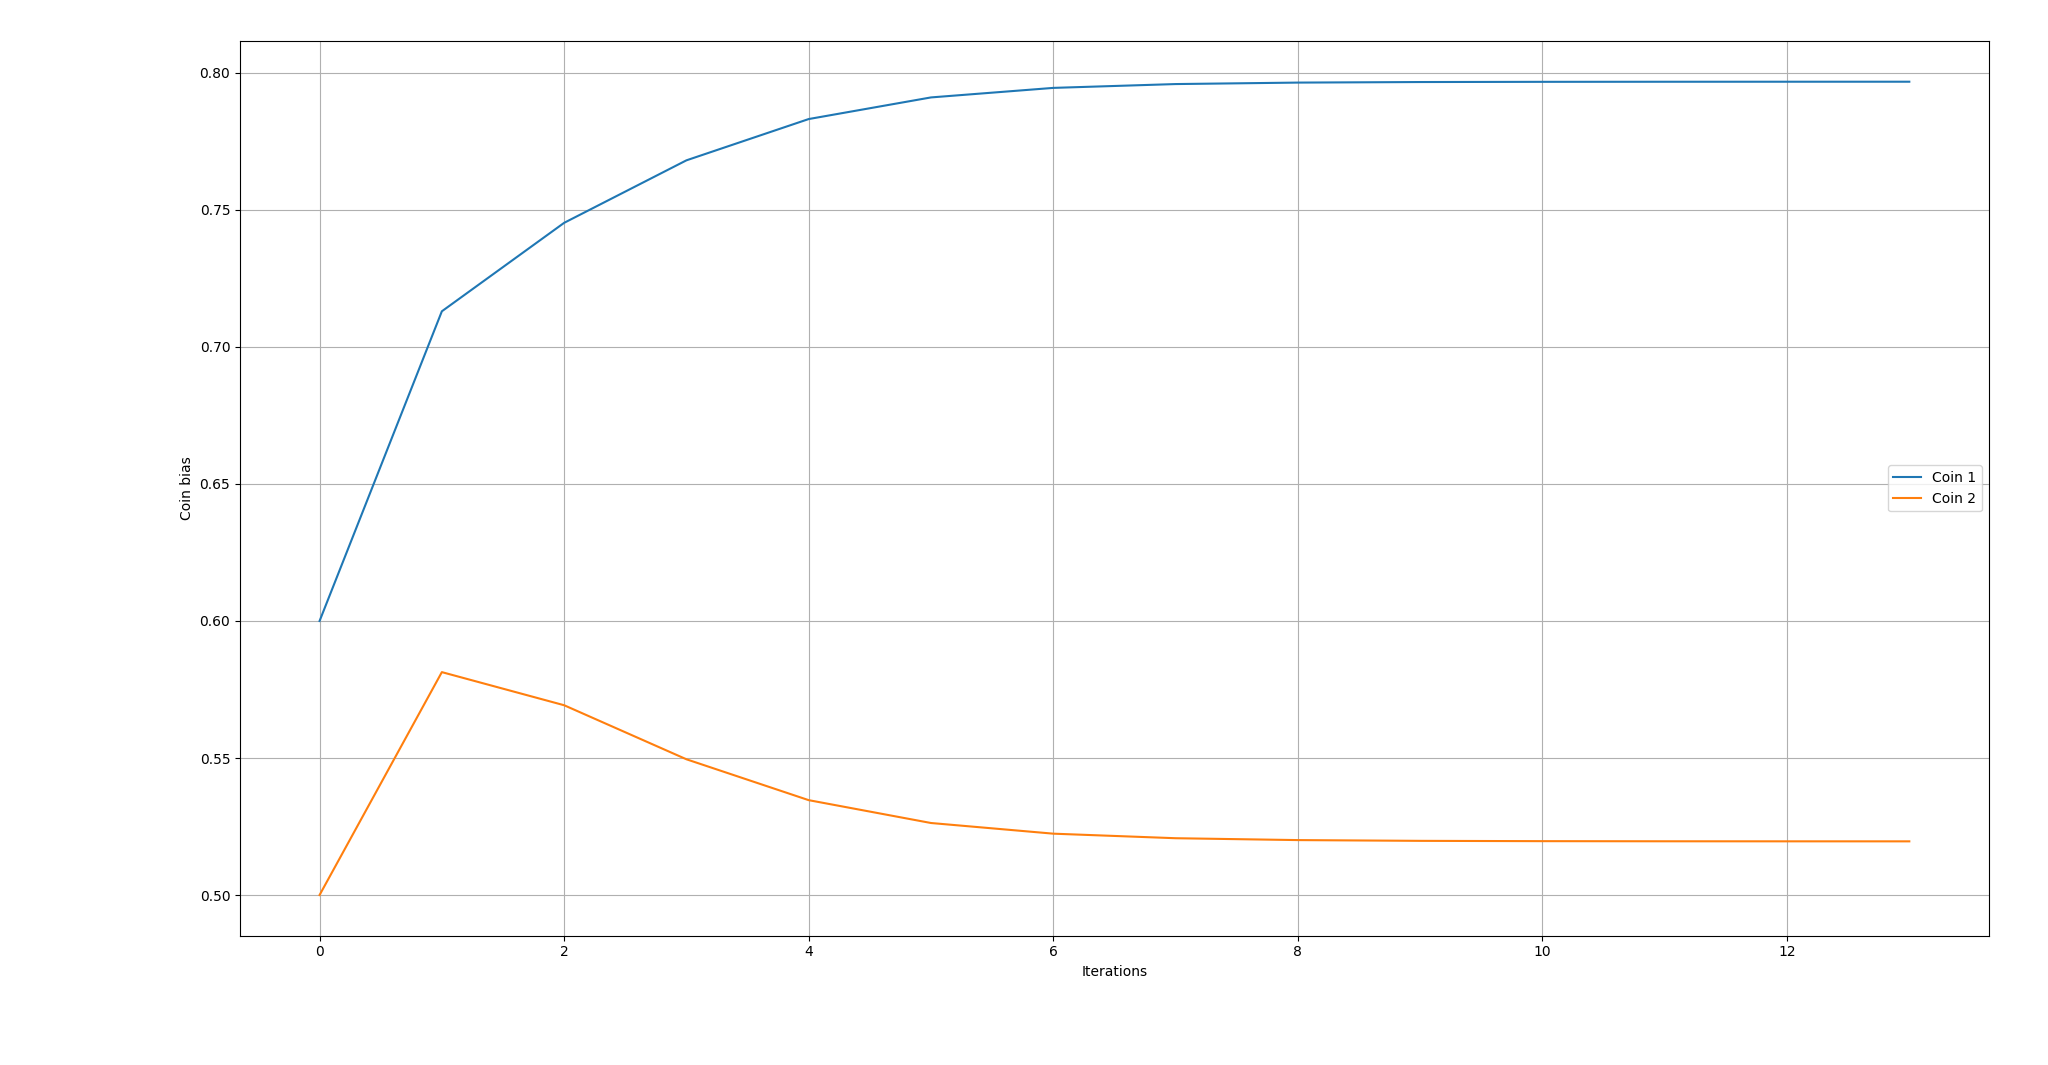
\includegraphics[width=\textwidth]{EM_Convergence}
\caption{Coin bias convergence curve using Expectation Maximization algorithm}
\label{em:conv}
\end{figure}
\textbf{VI.} In contrast, variational inference (Bayes in general) uses the underlaying prior distribution of the parameters. These can be further modeled with the additional distributions, or as we have done in our solution, initialized using hyperparameters. The result of the Variational Inference algorithm contains not only the most probable solution but also the information about confidence in the calculated values. Figure \ref{vi:conv} shows how confidence in the values grows as we increase number of iterations.
\begin{figure}[H]
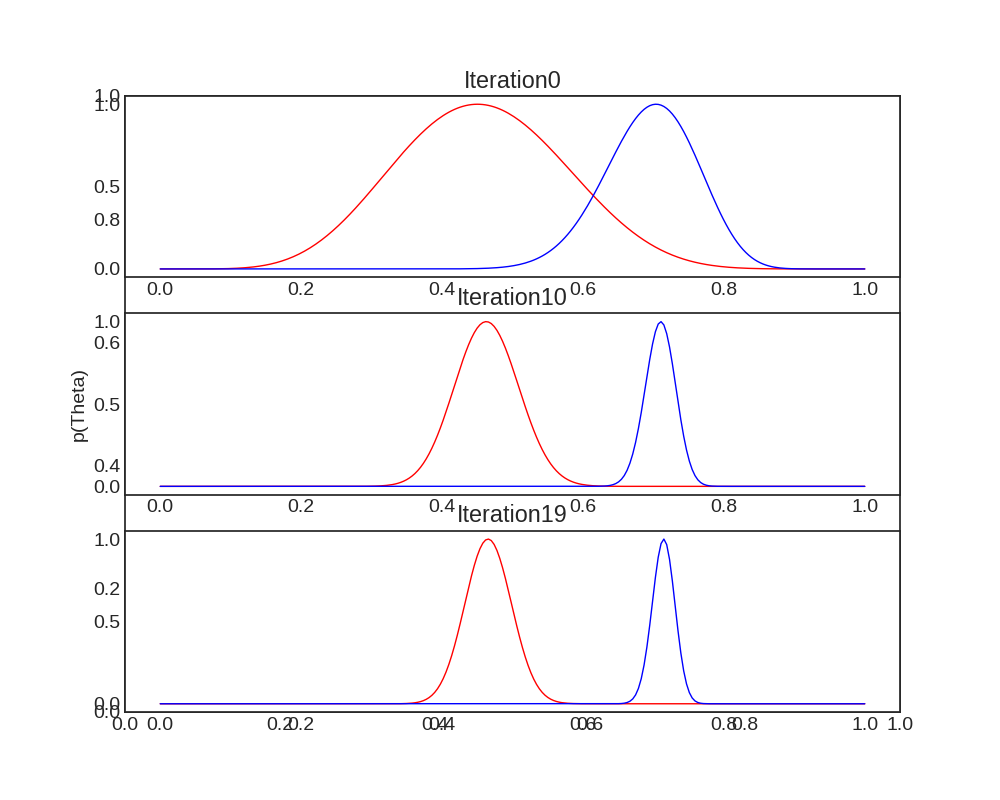
\includegraphics[width=\textwidth]{VI_Convergence}
\caption{Coin bias convergence curve using Variational Inference algorithm}
\label{vi:conv}
\end{figure}
\begin{table}
\csvautotabular{responsibilities.csv}
\caption {Coin responsibilities}
\label{resp:conv}
\end{table}
\textbf{Responsibilities.} Also, we have modeled the distribution of the K components, therefore we can track how expected values of the classes converge to their real values. This is show using the Table \ref{resp:conv} for the same iteration steps as in Figure \ref{vi:conv}. We call this responsibilities, because it shows us the probability that the coin $k$ (columns) is responsible for the event $n$ (rows) in the iteration $i$ of the algorithm.
\begin{figure}[H]
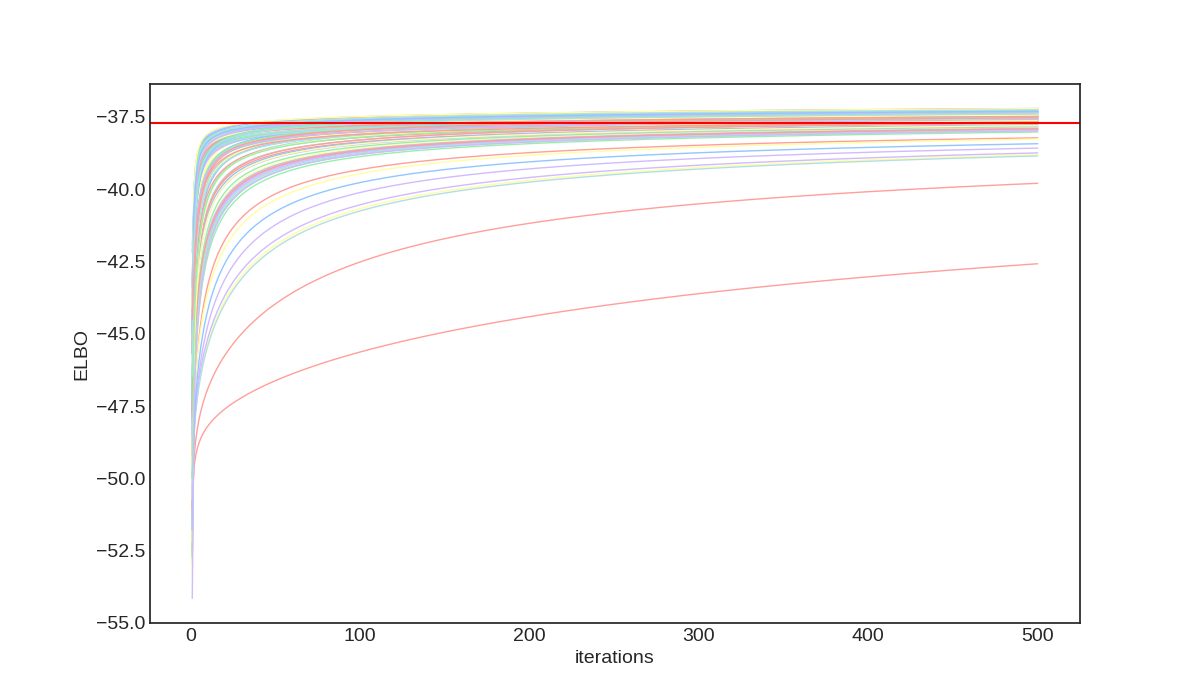
\includegraphics[width=\textwidth]{ELBO_Convergence}
\caption{Different initializations converge to different local optima of the ELBO}
\label{elbo:conv}
\end{figure}
\textbf{Initialization.} The ELBO is generally a non-convex objective function. Convergence to the local optimum is guaranteed, however, it can be sensitive with regard to the initialization. Figure \ref{elbo:conv} shows the ELBO convergence for 100 random initializations of the model parameters. Red line denotes the average of the convergence asymptote for all runs. 
\textbf{Convergence.} We define the treshold for the change of ELBO value between subsequent algorithm iterations. Once this difference has fallen under the treshold the procedure stops.
\textbf{Calculation}. During the calculation of the coefficient (which may grow arbitrarily large) we have encountered the problems with the calculation of the normalization coefficient for Dirichlet distribution. Replacing the hand-crafted version with the one from \textit{scipy} package resolved the problem.
\section{Conclusion}
We described variational inference algorithm with mean-field approximation. Update equations for a simple mixture models were derived. Evidence lower bound optimization procedure was used as a criteria for algorithm convergence. We have choosen probability distribution from exponential family with conjugate priors in order to simplify the mathematical model construction.
\end{document}
